\documentclass[11pt,a4paper]{article}
\usepackage[T1]{fontenc}
\usepackage[utf8]{inputenc}
\usepackage{lmodern}
\usepackage{amsmath,amssymb,amsthm,mathtools,mathrsfs}
\usepackage{graphicx,float,xcolor,multicol}
\usepackage[shortlabels]{enumitem}
\usepackage[margin=27mm]{geometry}
\usepackage{microtype,needspace,placeins}
\usepackage{tikz,tikz-cd}
\usetikzlibrary{arrows.meta,calc,positioning,patterns,decorations.pathreplacing}
\usepackage[colorlinks=true,linkcolor=teal,urlcolor=teal,citecolor=teal]{hyperref}
\setlength{\parindent}{0pt}
\setlength{\parskip}{.6em}
\setcounter{secnumdepth}{0}
\allowdisplaybreaks
\raggedbottom
\providecommand{\cross}{\times}
\DeclareUnicodeCharacter{2020}{\ensuremath{\dagger}}
\DeclareMathOperator{\supp}{supp}
\DeclareMathOperator*{\esssup}{ess\,sup}
\providecommand{\chapter}{\section}
\newenvironment{tool}[2]{\subsection*{Tool #1 --- #2}}{}
\newcommand{\ToolRef}[1]{Tool #1}
\newcommand{\FigureTag}[2]{\textit{Figure #1}}
\newcommand{\Result}[1]{\subsection*{#1}}
\newcommand{\Application}[1]{\subsubsection*{Application\if\relax\detokenize{#1}\relax\else\space--- #1\fi}}
\newcommand{\ProofHeading}{\par\textit{Proof.}\space}
\newcommand{\ProofOf}[1]{\par\textit{Proof of #1.}\space}
\newcommand{\RemarkHeading}{\par\textbf{Remark.}\space}
\newcommand{\NoteHeading}{\par\textbf{Note.}\space}
\newcommand{\ExerciseHeading}{\par\textbf{Exercise.}\space}

% Rendering support only; mathematical text is in each independent post.
\usepackage{booktabs,array,longtable}
\definecolor{HandoutBlue}{HTML}{2F6690}
\definecolor{HandoutNavy}{HTML}{17365D}
\newtheorem{theorem}{Theorem}
\newtheorem{lemma}[theorem]{Lemma}
\newtheorem{proposition}[theorem]{Proposition}
\newtheorem{corollary}[theorem]{Corollary}
\newtheorem{conjecture}[theorem]{Conjecture}
\newtheorem{definition}{Definition}
\newtheorem{example}{Example}
\newtheorem{namedtoolcounter}{Tool}
\newenvironment{namedtool}[1]{\begin{namedtoolcounter}[#1]}{\end{namedtoolcounter}}
\newtheorem*{claim}{Claim}
\newtheorem*{remark}{Remark}
\newtheorem*{exercise}{Exercise}
\newtheorem*{question}{Question}
\newtheorem*{observation}{Observation}
\newcommand{\SourceChapter}[2]{\section*{#2}}
\newcommand{\Lecture}[2]{\section*{Lecture #1: #2}}
\newcommand{\unclear}[1]{\textit{[unclear: #1]}}
\newcommand{\sourcegap}{\textit{[unfinished in the source]}}
\DeclareMathOperator{\dist}{dist}
\DeclareMathOperator{\id}{id}
\DeclareMathOperator{\Hol}{Hol}
\DeclareMathOperator{\Per}{Per}
\DeclareMathOperator{\Fix}{Fix}
\DeclareMathOperator{\diam}{diam}
\DeclareMathOperator{\Var}{Var}
\DeclareMathOperator{\Leb}{Leb}
\DeclareMathOperator{\Hom}{Hom}
\DeclareMathOperator{\End}{End}
\DeclareMathOperator{\Ann}{Ann}
\DeclareMathOperator{\Spec}{Spec}
\DeclareMathOperator{\Max}{Max}
\DeclareMathOperator{\Ob}{Ob}
\DeclareMathOperator{\Tor}{Tor}
\DeclareMathOperator{\Ass}{Ass}
\DeclareMathOperator{\Mor}{Mor}
\DeclareMathOperator{\Fun}{Fun}
\DeclareMathOperator{\Nat}{Nat}
\DeclareMathOperator{\Cone}{Cone}
\DeclareMathOperator{\MCG}{MCG}
\DeclareMathOperator{\Aut}{Aut}
\DeclareMathOperator{\Deck}{Deck}
\DeclareMathOperator{\SL}{SL}
\DeclareMathOperator{\PSL}{PSL}
\DeclareMathOperator{\Area}{Area}
\DeclareMathOperator{\im}{im}
\DeclareMathOperator{\PSh}{PSh}
\newcommand{\CRing}{\mathsf{CRings}}
\newcommand{\AMod}{A\text{-}\mathsf{Mod}}
\newcommand{\Ab}{\mathsf{Ab}}
\newcommand{\Z}{\mathbb Z}
\newcommand{\Q}{\mathbb Q}
\newcommand{\R}{\mathbb R}
\newcommand{\C}{\mathbb C}
\newcommand{\N}{\mathbb N}
\newcommand{\kk}{\mathbb k}
\renewcommand{\aa}{\mathfrak a}
\newcommand{\bb}{\mathfrak b}
\newcommand{\pp}{\mathfrak p}
\newcommand{\qq}{\mathfrak q}
\newcommand{\mm}{\mathfrak m}
\newcommand{\nn}{\mathfrak n}
\newcommand{\rad}{\mathrm r}
\newcommand{\cat}[1]{\mathsf{#1}}
\setcounter{secnumdepth}{0}
\allowdisplaybreaks

% Notation used only by the newly added notes.
\setlength{\emergencystretch}{2em}
\providecommand{\D}{\mathbb D}
\providecommand{\M}{\mathcal M}
\providecommand{\Chat}{\widehat{\mathbb C}}
\providecommand{\Crit}{\operatorname{Crit}}
\providecommand{\Int}{\operatorname{Int}}
\providecommand{\Ext}{\operatorname{Ext}}

\graphicspath{{figures/smooth-covering-manifolds/}}
\begin{document}
\section*{Smooth Covering Manifolds}
% BLOG-CONTENT-BEGIN
\section{Coverings and smooth structures}

\subsection{The lifted smooth structure}
\setcounter{definition}{0}\begin{definition}[Smooth covering]
A topological covering map $p:E\to M$ is said to be a \emph{smooth covering map} if, for every $x\in M$, there is an evenly covered neighbourhood $U_x$ of $x$ with
\[
 p^{-1}(U_x)=\bigsqcup_{\alpha\in I}V_\alpha,
 \qquad p|_{V_\alpha}:V_\alpha\longrightarrow U_x
 \quad\text{a diffeomorphism for every }\alpha\in I.
\]
\end{definition}

\setcounter{theorem}{0}\begin{proposition}\label{prop:lift-smooth}
Let $M$ be a smooth $n$-manifold, $E$ a connected topological space, and $p:E\to M$ a topological covering map. Then $E$ admits a unique smooth structure which makes it a smooth $n$-manifold and makes $p$ a smooth covering map.
\end{proposition}
\textbf{Hausdorffness.} It is easy to see that $E$ is Hausdorff. Let $e_1,e_2\in E$. If $p(e_1)\ne p(e_2)$, then the Hausdorff property of $M$ separates $p(e_1)$ and $p(e_2)$ by neighbourhoods which can be pulled back to $E$. If $p(e_1)=p(e_2)$, then the covering-map definition separates $e_1$ and $e_2$: let $\widetilde p=p(e_1)=p(e_2)$ and let $U_{\widetilde p}$ be an evenly covered neighbourhood of $\widetilde p$. Then $e_1$ and $e_2$ must belong to different slices of $p^{-1}(U_{\widetilde p})$. Hence $E$ is Hausdorff.
% The source writes p(e_1),p(e_2) in the separation sentence of Case II;
% e_1,e_2 is the clear local label typo, as its next sentence explicitly states.
\begin{figure}[H]
 \centering
 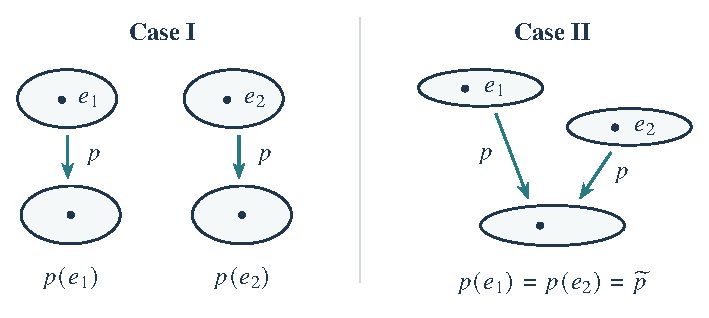
\includegraphics[width=.78\linewidth,height=5.2cm,keepaspectratio]{sc-fig-01.pdf}
 \FigureTag{SC1}{fig:sc-01}
\end{figure}

\paragraph{Compatible charts.}
Now let us dress $E$ with a smooth structure. Let $y\in E$, put $x=p(y)$, and let $U_x$ be an evenly covered neighbourhood of $x$. Let $(\varphi,U'_x)$ be a chart containing $x$, so $x\in U'_x$. Shrink $U_x$ (or $U'_x$) to $U_x\cap U'_x=U$. Then $(\varphi,U)$ is still a chart, and $U$ is still an evenly covered neighbourhood of $x$.

Write $p^{-1}(U)=\bigsqcup_{\alpha\in I}V_\alpha$. Say $y\in V_\alpha$; then $(V_\alpha,\varphi\circ p|_{V_\alpha})$ is a chart for $E$. These charts are compatible. Let $(\widetilde V,\widetilde\varphi)$ and $(\widetilde W,\widetilde\psi)$ be two such charts for $E$. The transition map is
\[
 \widetilde\psi\circ\widetilde\varphi^{-1}:
 \widetilde\varphi(\widetilde V\cap\widetilde W)
 \longrightarrow\widetilde\psi(\widetilde V\cap\widetilde W).
\]
Here $\widetilde\psi=\psi\circ p|_{\widetilde W}$ and $\widetilde\varphi=\varphi\circ p|_{\widetilde V}$, where $(p(\widetilde W),\psi)$ and $(p(\widetilde V),\varphi)$ are charts of $M$.
Consequently,
\begin{align*}
 \widetilde\psi\circ\widetilde\varphi^{-1}
 &=\left(\widetilde\psi|_{\widetilde V\cap\widetilde W}\right)
   \circ\widetilde\varphi^{-1}|_{\widetilde\varphi(\widetilde V\cap\widetilde W)}\\
 &=\left(\psi\circ p|_{\widetilde V\cap\widetilde W}\right)
   \circ\left(\varphi\circ p|_{\widetilde V}\right)^{-1}
   |_{\widetilde\varphi(\widetilde V\cap\widetilde W)}\\
 &=\left(\psi\circ p|_{\widetilde V\cap\widetilde W}\right)
   \circ\left(\varphi\circ p|_{\widetilde V\cap\widetilde W}\right)^{-1}\\
 &=\psi\circ p|_{\widetilde V\cap\widetilde W}
   \circ\left(p|_{\widetilde V\cap\widetilde W}\right)^{-1}\circ\varphi^{-1}
  =\psi\circ\varphi^{-1}.
\end{align*}

\paragraph{Smoothness of the covering map.}
Another immediate fact is that, with this smooth structure, $p$ is a smooth map. Let $y\in E$ and $x=p(y)$, let $(\varphi,U)$ be the evenly covered chart of $M$, and let $(\widetilde\varphi,V)$ be the corresponding chart of $E$, as constructed before. Then $p(V)\subseteq U$; in fact, $p(V)=U$. We have
\[
 \varphi\circ p\circ\widetilde\varphi^{-1}
 =\varphi\circ p\circ(\varphi\circ p)^{-1}=\id,
\]
which is smooth from $\widetilde\varphi(V)$ to $\varphi(U)$. Thus $p$ is a smooth covering map. What we have in particular managed to prove here is that $p|_V:V\to U$ is smooth; one can similarly prove that the inverse branch $p^{-1}|_U:U\to V$ is smooth.

\subsection{Countability of the fundamental group}
\setcounter{theorem}{1}\begin{lemma}[Countability of the fundamental group]\label{lem:countable-fundamental}
Let $M$ be a topological manifold. Then $\pi_1(M,P)$ is countable for every $P\in M$.
\end{lemma}

\subsection{Proper local diffeomorphisms}

\setcounter{theorem}{2}\begin{proposition}\label{prop:proper-cover}
Let $M$ be a connected smooth manifold and let $p\colon E\to M$ be a proper local diffeomorphism. Then $p$ is a covering map.
\end{proposition}

\begin{proof}
The image $p(E)$ is open because $p$ is a local diffeomorphism. It is also closed because $p$ is proper and $M$ is locally compact and Hausdorff. Since $M$ is connected, $p$ is surjective.

Since $p$ is a local diffeomorphism, $p^{-1}(\{q\})$ is discrete. It is also compact, because $p$ is proper, and hence is finite. Write $p^{-1}(q)=\{p_i\}_{i=1}^{n}$. For each pair $p_i,q$, there are open neighbourhoods $V_i$ and $U_i$ of $p_i$ and $q$, respectively, such that $p|_{V_i}\colon V_i\to U_i$ is a diffeomorphism.

Since $E$ is Hausdorff, there are neighbourhoods $W_i$ of $p_i$ such that $W_i\cap W_j=\varnothing$ whenever $i\ne j$. Replace $V_i$ by $V_i\cap W_i$ and $U_i$ by $p|_{V_i}(V_i\cap W_i)$. The restriction $p|_{V_i}\colon V_i\to U_i$ is again a diffeomorphism.

Now replace each $U_i$ by $U=\bigcap_{i=1}^{n}U_i$ and each $V_i$ by $V_i\cap(p|_{V_i})^{-1}(U)$. Then $p|_{V_i}\colon V_i\to U$ is a diffeomorphism for every $i$, and $V_i\cap V_j=\varnothing$ for $i\ne j$.

The set $K=\bigl(\bigcup_{i=1}^{n}V_i\bigr)^c$ is closed in $E$, so $p(K)$ is closed. Replace $U$ by $U\setminus p(K)$.

Then $p^{-1}(U)\subseteq\bigcup_{i=1}^{n}V_i$. Finally, replace $V_i$ by $V_i\cap p^{-1}(U)$. After these shavings, we have
\[
p^{-1}(U)=\bigsqcup_{i=1}^{n}V_i,
\qquad p|_{V_i}\colon V_i\longrightarrow U
\quad\text{a diffeomorphism}.
\]
Thus $p$ is a smooth covering map.
\end{proof}

\subsection{Covering Lie groups}

Now let us impose further structures on our original setting and see where it leads us. We then saw how the structure was still preserved once we shifted our course to the category of smooth manifolds. More precisely, we saw that a topological cover of a manifold also preserves the smooth structure. If we now lift this to the category of Lie groups and ask whether smooth covering maps preserve the group structure, the following proposition answers this in its full glory!

\setcounter{theorem}{3}\begin{proposition}[Yes, group structure is preserved!]\label{prop:lie-group}
Let $G$ be a connected Lie group, and let $\pi\colon\widetilde{G}\to G$ be a smooth covering map with $\widetilde{G}$ simply connected. Then one can endow $\widetilde{G}$ with a Lie group structure for which $\pi$ is a Lie group homomorphism. Furthermore, $\widetilde{G}$ is unique up to Lie group isomorphism.
\end{proposition}
% BLOG-CONTENT-END
\end{document}
